% This is samplepaper.tex, a sample chapter demonstrating the
% LLNCS macro package for Springer Computer Science proceedings;
% Version 2.21 of 2022/01/12
%
\documentclass{llncs}

% ========================
% Vietnamese support
% ========================
\usepackage[T5]{fontenc}
\usepackage[utf8]{inputenc}
\usepackage[vietnamese,english]{babel}
% pdflatex-compatible Vietnamese setup using UTF-8 input and T5 font encoding.
%

\usepackage{graphicx}
\usepackage{url}
\usepackage{booktabs}
\usepackage{array}
\usepackage{subcaption}
\usepackage{placeins}
\usepackage[font=small,labelfont=bf]{caption}
\graphicspath{{figures/}}
\setlength{\textfloatsep}{12pt plus 2pt minus 2pt}
\setlength{\floatsep}{10pt plus 2pt minus 2pt}
\setlength{\intextsep}{10pt plus 2pt minus 2pt}
\renewcommand{\arraystretch}{1.12}
\renewcommand{\topfraction}{0.9}
\renewcommand{\bottomfraction}{0.8}
\renewcommand{\textfraction}{0.08}
\renewcommand{\floatpagefraction}{0.8}
% Used for displaying figures. This sample uses an inline placeholder box
% so the document can compile even when no external image file is present.
%

% If you use the hyperref package, please uncomment the following two lines
% to display URLs in blue roman font according to Springer's eBook style:
%\usepackage{color}
%\renewcommand\UrlFont{\color{blue}\rmfamily}
%\urlstyle{rm}
%
\begin{document}
%
\title{SISTAR: An Efficient DDoS Detection and Mitigation Framework Utilizing Programmable Data Planes}
%
%
\author{Đặng Minh Tú\inst{1,2}\and
Võ Quang Vũ\inst{1,2} \and
Nghi Hoàng Khoa\inst{1,2}}
%
%
\institute{Khoa Mạng máy tính và Truyền thông \and
Trường Đại học Công nghệ Thông tin, ĐHQG-HCM
\email{\{24520033,24522045\}@gm.uit.edu.vn} \email{khoanh@uit.edu.vn}}
%
\maketitle              % typeset the header of the contribution
\pagestyle{plain}
%
\begin{abstract}
Bài viết này trình bày một nghiên cứu tái hiện rút gọn ý tưởng của SISTAR, một khuôn khổ phát hiện và giảm thiểu tấn công DDoS dựa trên các mô hình học máy nhẹ có khả năng triển khai trong programmable data plane. Thay vì lặp lại nội dung của bài báo gốc, nghiên cứu tập trung xây dựng một quy trình thực nghiệm bằng Python để đánh giá ba mô hình DT, RF và DT-CTS trên tập CICIDS2017 đã được chuẩn hóa, đồng thời sử dụng số lượng threshold như một đại diện cho chi phí triển khai trên switch. Trên cơ sở đó, nghiên cứu đề xuất thêm một cơ chế giảm thiểu mới mang tên hierarchical confidence-aware pushback. Cơ chế này kết hợp edge detector, core detector và suspicion score để điều phối phản ứng theo nhiều mức, từ giám sát tới chặn hoàn toàn khi bằng chứng đã đủ mạnh. Kết quả thực nghiệm cho thấy DT-CTS vẫn duy trì chất lượng phân loại cạnh tranh trong khi giảm đáng kể số threshold so với DT thông thường. Đồng thời, cơ chế pushback đề xuất giúp suy giảm gần như toàn bộ attack bytes tới victim mà vẫn tránh được false block trong mô phỏng, qua đó cho thấy hiệu quả tốt hơn so với chiến lược block ngay sau một lần phát hiện malicious.

\keywords{DDoS detection \and programmable data plane \and DT-CTS \and pushback \and CICIDS2017}
\end{abstract}
%
%
%
\section{Tổng quan}

Tấn công từ chối dịch vụ phân tán (Distributed Denial of Service -- DDoS) vẫn là một trong những bài toán khó và thực tế nhất trong an toàn mạng. Vấn đề không chỉ là phát hiện đúng lưu lượng độc hại, mà còn phải phản ứng đủ sớm để giảm tải cho các liên kết và thiết bị trung gian trước khi traffic tấn công chạm tới máy chủ đích. Nếu mọi quyết định đều được đưa ra ở máy chủ hoặc bộ điều khiển trung tâm, hệ thống có thể phân tích khá chính xác nhưng vẫn chậm về mặt vận hành.

SISTAR được đề xuất để xử lý chính mâu thuẫn đó. Ý tưởng của hệ thống là phát hiện DDoS ngay trong mạng bằng các mô hình cây quyết định nhẹ, sau đó dùng cơ chế pushback để đẩy hành động giảm thiểu về phía upstream switch, tức là gần nguồn tấn công hơn. Trong bối cảnh programmable data plane và P4 ngày càng được quan tâm, hướng tiếp cận này có ý nghĩa rõ ràng vì nó nối được hai phía: học máy và khả năng xử lý trực tiếp ở lớp chuyển tiếp gói tin.

Báo cáo này không nhằm dịch lại bài báo gốc. Thay vào đó, nhóm chọn cách tái hiện những ý chính của SISTAR bằng một workflow phần mềm có thể chạy lại được. Toàn bộ phần trình bày tập trung vào ba câu hỏi sau:
\begin{enumerate}
\item Mô hình học máy nào đủ chính xác để phân biệt benign flow và attack flow?
\item Mô hình nào đủ gọn để có tiềm năng triển khai trong data plane, với số lượng threshold nhỏ?
\item Một cơ chế pushback mới có thể giữ được hiệu quả chặn attack nhưng giảm block nhầm benign traffic hay không?
\end{enumerate}

Để trả lời các câu hỏi này, nhóm xây dựng một pipeline gồm tiền xử lý dữ liệu CICIDS2017, huấn luyện ba mô hình DT, RF và DT-CTS, đánh giá độ chính xác và số threshold, sau đó mô phỏng ba chính sách giảm thiểu: no pushback, immediate pushback và hierarchical confidence-aware pushback. Kết quả thu được cho thấy phần cải tiến của nhóm có ý nghĩa ở cấp độ hệ thống, chứ không chỉ dừng ở việc thay đổi một mô hình phân loại.

\section{Giới thiệu}

Các hệ thống phòng thủ DDoS hiện nay thường phải đánh đổi giữa hai mục tiêu: độ chính xác trong phát hiện và tốc độ phản ứng trong vận hành. Những hướng tiếp cận dựa hoàn toàn vào máy chủ phân tích tập trung có ưu điểm là linh hoạt, nhưng tại thời điểm hệ thống có thể kết luận một nguồn lưu lượng là độc hại thì phần lớn traffic tấn công đã đi qua mạng. Theo chiều ngược lại, nếu logic phát hiện được đưa xuống switch hoặc data plane, mô hình phải đủ gọn, đủ đơn giản và có thể biểu diễn dưới dạng các điều kiện so sánh ngưỡng \cite{bosshart2014p4,breiman2001random}.

SISTAR là một hướng tiếp cận đáng chú ý vì sử dụng các mô hình cây quyết định, đặc biệt là DT-CTS, để thu hẹp khoảng cách giữa học máy và programmable data plane. Về bản chất, DT-CTS chủ động khống chế số lượng threshold trên mỗi feature nhằm tạo điều kiện thuận lợi hơn cho việc ánh xạ mô hình thành rule và thanh ghi trên switch so với cây quyết định thông thường. Trong nghiên cứu này, số lượng threshold được sử dụng như một chỉ báo thực dụng cho độ phức tạp triển khai.

Tuy nhiên, một hệ thống chỉ phát hiện tốt là chưa đủ. Nếu cơ chế giảm thiểu được triển khai quá quyết liệt, chẳng hạn block ngay sau một lần dự đoán malicious, hệ thống có thể suy giảm attack traffic rất nhanh nhưng đồng thời cũng làm tăng nguy cơ chặn nhầm benign traffic. Đây là điều không mong muốn trong môi trường thực tế, nơi những burst hợp lệ hoặc các đợt tăng lưu lượng ngắn hạn vẫn có thể xuất hiện.

\subsection{Kiến trúc SISTAR và động lực cải tiến}

Từ những quan sát trên, nghiên cứu không chỉ tái hiện phần phân loại của SISTAR mà còn mở rộng sang cơ chế điều phối giảm thiểu. Một policy mới mang tên hierarchical confidence-aware pushback được xây dựng, trong đó quyết định chặn không dựa trên một dự đoán đơn lẻ mà dựa trên bằng chứng được tích lũy từ nhiều detector theo thời gian. Cách tiếp cận này cho phép hệ thống phản ứng theo nhiều mức độ, thay vì chỉ có hai trạng thái là cho qua hoặc block ngay.

Trước khi trình bày chi tiết quy trình tái hiện, cần nhìn lại kiến trúc hệ thống của SISTAR để làm rõ bối cảnh mà phần cải tiến được xây dựng trên đó.

\begin{figure}
\centering
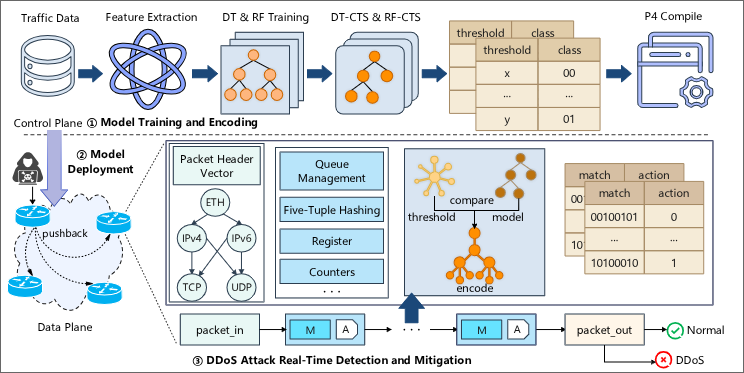
\includegraphics[width=0.88\textwidth]{image.png}
\caption{Sơ đồ hệ thống SISTAR theo kiến trúc gốc: phát hiện được đưa vào trong mạng và kết hợp với cơ chế pushback để chặn lưu lượng sớm hơn ở phía upstream.}
\label{fig:sistar-system}
\end{figure}

Hình~\ref{fig:sistar-system} thể hiện tinh thần cốt lõi của SISTAR: switch không chỉ thực hiện chức năng chuyển tiếp mà còn tham gia vào phát hiện và phối hợp giảm thiểu. Khi một vùng mạng phát hiện lưu lượng đáng nghi, hành động lọc không nhất thiết phải chờ tới victim mà có thể được đẩy ngược lên upstream switch để giảm tải sớm hơn trên toàn tuyến.

\subsection{Đóng góp của nghiên cứu}

Đóng góp chính của nghiên cứu có thể tóm tắt như sau:
\begin{enumerate}
\item Xây dựng lại một pipeline thực nghiệm gọn, bám theo tinh thần của SISTAR trên tập CICIDS2017 với ba mô hình DT, RF và DT-CTS, kèm các chỉ số accuracy, F1 và threshold count.
\item Đề xuất cơ chế hierarchical confidence-aware pushback gồm edge detector, core detector và suspicion score để hệ thống leo thang phản ứng qua các mức monitor, local rate-limit, upstream pushback và hard block.
\item Chứng minh bằng thực nghiệm rằng cơ chế cải tiến này tạo được cân bằng tốt hơn giữa suy giảm attack traffic và hạn chế false block so với immediate pushback trong cùng một môi trường mô phỏng.
\end{enumerate}

\section{Các nghiên cứu liên quan}

Các công trình liên quan đến đề tài này có thể chia thành ba nhóm chính: phát hiện DDoS bằng học máy trên dữ liệu flow, triển khai logic xử lý trong programmable data plane, và các cơ chế pushback nhằm chặn lưu lượng càng gần nguồn càng tốt.

Ở nhóm thứ nhất, các bộ dữ liệu như CICIDS2017 được sử dụng rộng rãi trong đánh giá phát hiện xâm nhập vì cung cấp nhiều kiểu DoS/DDoS trong môi trường mô phỏng doanh nghiệp \cite{sharafaldin2018cicids}. Với dữ liệu dạng flow, cây quyết định và random forest là hai lựa chọn quen thuộc vì chi phí suy luận thấp hơn nhiều mô hình sâu và cũng dễ diễn giải hơn \cite{breiman2001random}. Tuy nhiên, nếu mục tiêu cuối cùng là đưa logic này xuống switch, random forest thường trở nên quá nặng do số rule và số threshold lớn.

Ở nhóm thứ hai, P4 và programmable data plane cho phép đưa một phần logic phân loại trực tiếp vào quá trình xử lý gói tin \cite{bosshart2014p4}. Đây là nền tảng khiến những hệ thống như SISTAR trở nên khả thi. Tuy nhiên, data plane vẫn có các ràng buộc rõ ràng về số bảng match, thanh ghi và loại phép toán hỗ trợ; do đó, mô hình có độ chính xác cao hơn chưa chắc đã là mô hình phù hợp hơn để triển khai.

Ở nhóm thứ ba, pushback là một ý tưởng đã được nghiên cứu từ lâu trong phòng thủ DDoS: thay vì chỉ drop traffic ở gần victim, quyết định lọc cần được đẩy lên upstream router hoặc switch để giải phóng tài nguyên mạng sớm hơn \cite{mahajan2002controlling}. Điểm mới của nghiên cứu này không nằm ở việc phát minh lại pushback, mà ở việc thiết kế lại policy ra quyết định theo hướng tích lũy độ tin cậy, thay vì block ngay khi có một lần phát hiện malicious.

\begin{table}[!htbp]
\caption{Tóm tắt ngắn gọn các hướng tiếp cận liên quan và vị trí của nghiên cứu này.}
\label{tab:sota}
\centering
\small
\setlength{\tabcolsep}{3pt}
\begin{tabular}{|p{2.2cm}|p{2.1cm}|p{2.2cm}|p{2.4cm}|p{2.2cm}|}
\hline
\textbf{Công trình / hướng} & \textbf{Mục tiêu chính} & \textbf{Mô hình / kỹ thuật} & \textbf{Ưu điểm} & \textbf{Hạn chế chính} \\
\hline
ML trên CICIDS2017 \cite{sharafaldin2018cicids,breiman2001random} & Phát hiện attack flow & DT, RF, mô hình học máy cổ điển & Dễ huấn luyện, dễ đo accuracy/F1 & Chưa giải quyết trực tiếp chi phí triển khai trên switch \\
\hline
Programmable data plane \cite{bosshart2014p4} & Xử lý lưu lượng ngay trong mạng & P4, rule-based pipeline & Phản ứng sớm, giảm phụ thuộc vào server & Bị ràng buộc bởi tài nguyên và kiểu phép toán hỗ trợ \\
\hline
Pushback truyền thống \cite{mahajan2002controlling} & Chặn lưu lượng gần nguồn & Upstream filtering / router cooperation & Giảm tải cho mạng phía sau & Dễ quá tay nếu quyết định chặn thiếu tin cậy \\
\hline
SISTAR gốc & Kết hợp ML nhẹ và pushback trong data plane & DT-CTS + pushback & Đưa phát hiện gần switch, giảm độ phức tạp mô hình & Chính sách block tức thời dễ làm tăng false block \\
\hline
Project này & Tái hiện SISTAR và cải tiến policy giảm thiểu & DT, RF, DT-CTS + hierarchical confidence-aware pushback & Cân bằng tốt hơn giữa giảm attack và giữ benign traffic & Mới dừng ở mô phỏng phần mềm, chưa đo trên phần cứng thật \\
\hline
\end{tabular}
\end{table}

Từ Bảng~\ref{tab:sota} có thể thấy khoảng trống mà nghiên cứu này hướng tới là sự kết hợp của hai yêu cầu: mô hình đủ nhẹ cho data plane và policy giảm thiểu đủ thận trọng để hạn chế block nhầm. Đây cũng là lý do phần cải tiến tập trung vào cơ chế pushback mới, thay vì thay thế hoàn toàn DT-CTS bằng một mô hình phức tạp hơn.

\FloatBarrier

\section{Phương pháp thực hiện}

\subsection{Mục tiêu thực nghiệm}

Pipeline thực nghiệm được xây dựng để kiểm tra đồng thời hai lớp vấn đề. Lớp thứ nhất là chất lượng phân loại giữa benign traffic và DDoS traffic. Lớp thứ hai là hiệu quả giảm thiểu khi đưa quyết định pushback vào chuỗi xử lý. Vì vậy, phương pháp của nhóm không chỉ dừng ở bước huấn luyện mô hình mà còn bao gồm cả phần mô phỏng phản ứng của mạng sau khi có kết quả phân loại.

\subsection{Dữ liệu và đặc trưng}

Nguồn dữ liệu chính của project là tập \texttt{combine.csv} được trích từ CICIDS2017 và chuẩn hóa về bài toán nhị phân: \texttt{BENIGN} và nhóm Wednesday DoS. Trong reproduction chính, hệ thống ưu tiên một số feature có liên hệ trực tiếp tới khả năng biểu diễn trong data plane, chẳng hạn \texttt{protocol}, \texttt{init\_win\_bytes\_forward}, \texttt{fwd\_header\_length}, \texttt{packet\_length\_mean} và \texttt{flow\_packets\_persecond}. Dữ liệu sau đó được ép kiểu số, xử lý \texttt{NaN}/\texttt{inf}, cắt bớt ngoại lai và chia train/test theo tỉ lệ 80/20.

\subsection{Ba mô hình được so sánh}

Ba mô hình được dùng trong toàn bộ thực nghiệm gồm:
\begin{enumerate}
\item \textbf{Decision Tree (DT):} baseline đơn giản, dễ hiểu, dễ chuyển thành các điều kiện dạng ``feature $\le$ threshold''.
\item \textbf{Random Forest (RF):} thường đạt chất lượng tốt nhưng số threshold lớn, do đó khó phù hợp với data plane.
\item \textbf{DT-CTS:} mô hình trọng tâm của project, giới hạn số threshold trên mỗi feature để giảm độ phức tạp triển khai.
\end{enumerate}

Ngoài accuracy, precision, recall và F1, project còn đo \textit{threshold count}. Chỉ số này không thay thế hoàn toàn các tài nguyên phần cứng như TCAM hay SRAM, nhưng là một đại diện hợp lý để so sánh footprint giữa các mô hình trong môi trường tái hiện phần mềm.

\subsection{Cơ chế hierarchical confidence-aware pushback}

Cải tiến chính của báo cáo nằm ở policy giảm thiểu mới. Thay vì block source ngay khi có một dự đoán attack, cơ chế này gán cho mỗi source một \textit{suspicion score}. Điểm số này tăng lên dựa trên các bằng chứng sau:
\begin{itemize}
\item edge detector dự đoán malicious,
\item core detector dự đoán malicious,
\item edge và core cùng đồng thuận,
\item traffic có dấu hiệu spike bất thường.
\end{itemize}

Song song với đó, suspicion score cũng giảm dần theo thời gian nếu source không tiếp tục có hành vi đáng nghi. Cách làm này giúp hệ thống không giữ trạng thái cảnh báo quá lâu chỉ vì một burst ngắn hạn.

Từ score hiện tại, hệ thống chọn một trong bốn mức phản ứng:
\begin{enumerate}
\item \texttt{monitor},
\item \texttt{local rate-limit},
\item \texttt{upstream pushback},
\item \texttt{hard block}.
\end{enumerate}

Mức phản ứng càng cao thì tỷ lệ traffic còn được forward tới victim càng thấp. Nói cách khác, pushback ở đây không còn là một quyết định nhị phân nữa, mà trở thành một quá trình leo thang có kiểm soát.

\begin{table}
\caption{Các thành phần chính của suspicion score và mức phản ứng trong policy mới.}
\label{tab:score-policy}
\centering
\begin{tabular}{p{3.0cm}p{2.2cm}p{4.6cm}}
\toprule
\textbf{Thành phần} & \textbf{Giá trị} & \textbf{Ý nghĩa} \\
\midrule
Edge evidence & +2 & Tín hiệu nghi ngờ sớm từ edge detector \\
Core evidence & +4 & Xác nhận mạnh hơn từ core detector \\
Agreement bonus & +3 & Tăng độ tin cậy khi edge và core cùng dự đoán attack \\
Spike evidence & +2 & Bổ sung bằng chứng khi traffic tăng đột biến \\
Decay & -1 / window & Giảm cảnh báo nếu source không tiếp tục đáng nghi \\
Monitor & score $\geq 3$ & Theo dõi, chưa cắt traffic \\
Local rate-limit & score $\geq 6$ & Giảm một phần traffic ở cục bộ \\
Upstream pushback & score $\geq 12$ & Đẩy hành động lọc về switch phía trước \\
Hard block & score $\geq 24$ + core=attack & Chặn hoàn toàn source khi bằng chứng đủ mạnh \\
\bottomrule
\end{tabular}
\end{table}

\subsection{Mô hình hệ thống và pipeline thực nghiệm}

\begin{figure}
\centering
\fbox{
\begin{minipage}{0.88\textwidth}
\vspace{0.2cm}
\centering
\textbf{Dataset CICIDS2017 subset}

$\Downarrow$

\textbf{Tiền xử lý và chọn feature}

$\Downarrow$

\textbf{Huấn luyện DT / RF / DT-CTS}

$\Downarrow$

\textbf{Đánh giá classification + threshold efficiency}

$\Downarrow$

\textbf{Sinh pushback trace theo source và time window}

$\Downarrow$

\textbf{Edge DT-CTS + Core DT-CTS + Spike signal}

$\Downarrow$

\textbf{Suspicion score}

$\Downarrow$

\textbf{Monitor $\rightarrow$ Local rate-limit $\rightarrow$ Upstream pushback $\rightarrow$ Hard block}
\vspace{0.2cm}
\end{minipage}
}
\caption{Pipeline thực nghiệm của project, từ phân loại tới mô phỏng giảm thiểu.}
\label{fig:pipeline}
\end{figure}

Hình~\ref{fig:pipeline} cho thấy logic tổng thể của hệ thống. Khác với cách trình bày thuần lý thuyết của bài báo gốc, pipeline trong project được tổ chức để có thể chạy lại hoàn toàn bằng mã nguồn Python, nhưng vẫn giữ đúng tinh thần ``phát hiện nhẹ, phản ứng sớm, giảm thiểu theo mức'' của SISTAR.

\begin{figure}
\centering
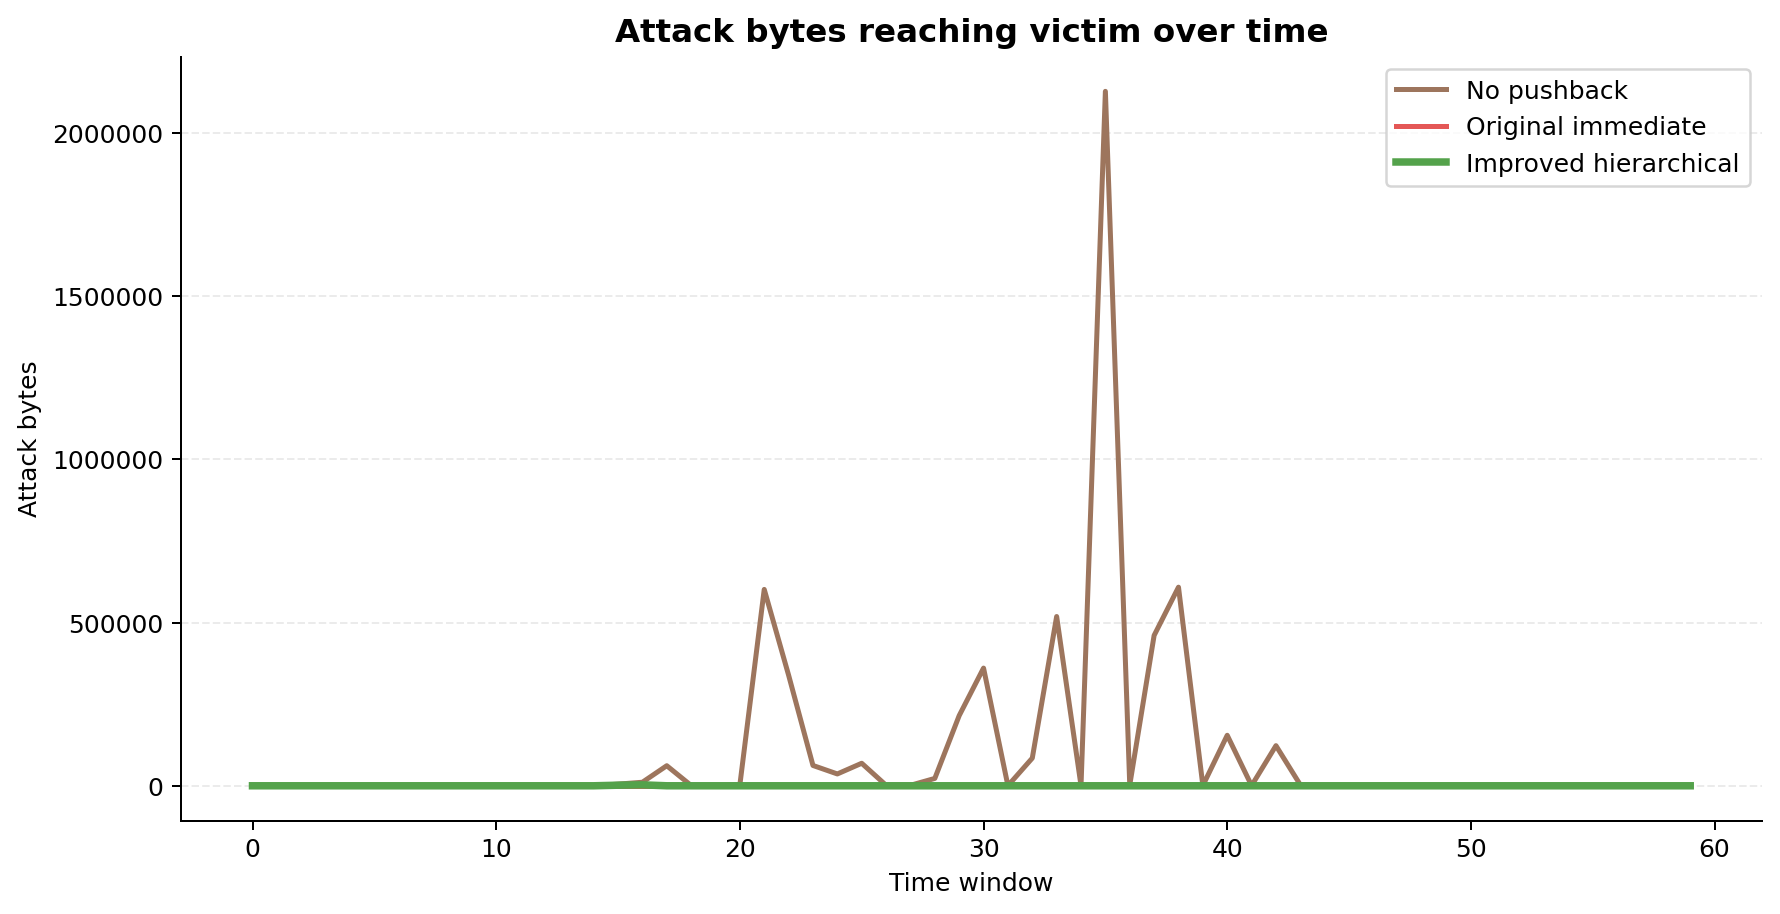
\includegraphics[width=0.9\textwidth]{figures/attack_timeline.png}
\caption{Diễn biến attack bytes tới victim theo thời gian giữa ba policy. Đường cong của hierarchical pushback bám sát immediate pushback về hiệu quả cắt attack, nhưng đạt được điều đó bằng cơ chế leo thang mềm hơn.}
\label{fig:attack-timeline}
\end{figure}

\section{Thử nghiệm và đánh giá}

\subsection{Thiết lập đánh giá}

Toàn bộ thực nghiệm chính được chạy trên workflow \texttt{reproduction/src/run\_full\_demo.py} và các script liên quan. Bộ dữ liệu được tách train/test theo tỉ lệ 80/20, sau đó ba mô hình DT, RF và DT-CTS được huấn luyện trên cùng một tập train để đảm bảo so sánh công bằng. Nhóm đánh giá theo hai hướng:
\begin{itemize}
\item \textbf{Chất lượng phân loại:} accuracy, precision, recall, F1.
\item \textbf{Hiệu quả triển khai và giảm thiểu:} threshold count, latency/FPR/FNR, attack bytes reaching victim, benign bytes preserved và false block events.
\end{itemize}

\subsection{Kết quả phân loại}

\begin{table}
\caption{So sánh kết quả phân loại của ba mô hình trong reproduction chính.}
\label{tab:classification-main}
\centering
\begin{tabular}{lcc}
\toprule
\textbf{Mô hình} & \textbf{Accuracy} & \textbf{F1} \\
\midrule
DT & 0.9901 & 0.9620 \\
RF & 0.9821 & 0.9327 \\
DT-CTS & 0.9800 & 0.9249 \\
\bottomrule
\end{tabular}
\end{table}

Kết quả reproduction chính cho thấy:
\begin{itemize}
\item DT đạt accuracy 0.9901 và F1 0.9620.
\item RF đạt accuracy 0.9821 và F1 0.9327.
\item DT-CTS đạt accuracy 0.9800 và F1 0.9249.
\end{itemize}

Nếu chỉ nhìn riêng F1 thì DT đang là mô hình tốt nhất trong lần chạy hiện tại. Tuy nhiên, điều đáng quan tâm hơn với mục tiêu của SISTAR là DT-CTS vẫn giữ chất lượng ở mức cạnh tranh trong khi được thiết kế để giảm số threshold. Đây mới là điểm quan trọng khi xét tới khả năng triển khai trên programmable switch, nơi chi phí bảng match và số điều kiện so sánh không thể bỏ qua.

\begin{figure}
\centering
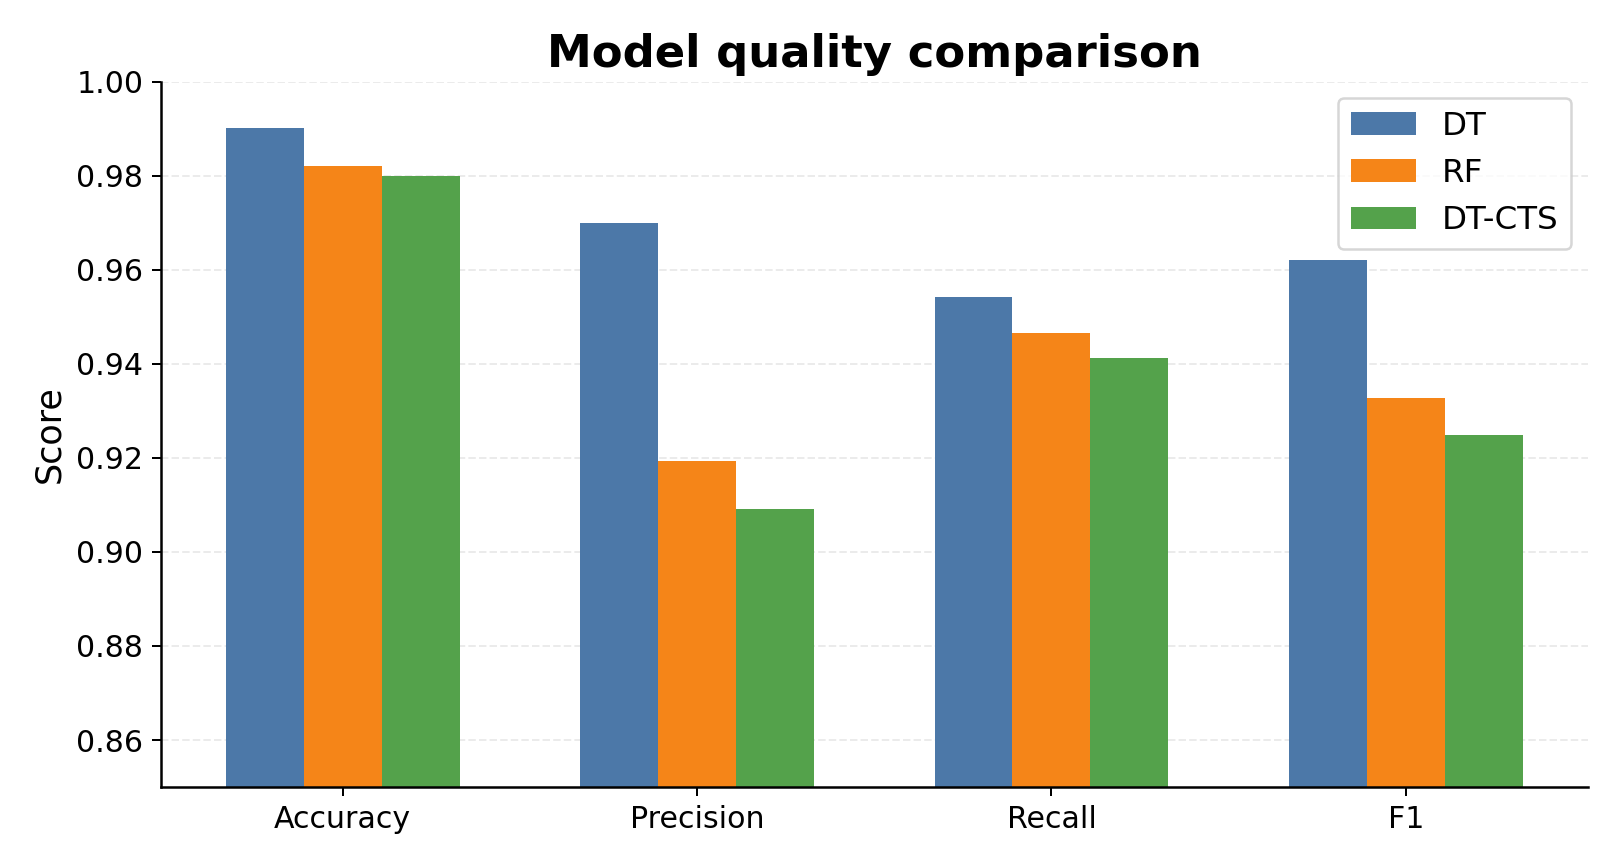
\includegraphics[width=0.78\textwidth]{figures/classification_metric_suite.png}
\caption{So sánh chất lượng phân loại của DT, RF và DT-CTS. DT-CTS thấp hơn nhẹ về F1, nhưng vẫn giữ khoảng cách nhỏ so với hai baseline trong khi hướng đến khả năng triển khai tốt hơn.}
\label{fig:classification-suite}
\end{figure}

\subsection{Hiệu quả theo số lượng threshold}

\begin{table}
\caption{So sánh footprint theo threshold giữa các mô hình chính.}
\label{tab:threshold-main}
\centering
\begin{tabular}{lp{2.1cm}p{4.7cm}}
\toprule
\textbf{Mô hình} & \textbf{Total thresholds} & \textbf{Nhận xét} \\
\midrule
DT & 36 & Baseline dễ hiểu nhưng còn khá nặng \\
RF & rất lớn & Khó phù hợp với data plane \\
DT-CTS & 14 & Giảm 61.11\% so với DT, phù hợp hơn cho switch \\
\bottomrule
\end{tabular}
\end{table}

Trong reproduction chính, DT dùng 36 threshold trong khi DT-CTS chỉ dùng 14 threshold, tương đương mức giảm khoảng 61.11\%. Ở benchmark paper-style với 3, 5 và 7 feature, cấu hình DT-CTS tốt nhất đạt F1 0.9614 với 14 threshold, và vẫn giảm 58.82\% số threshold so với DT cùng cấu hình. Kết quả này cho thấy DT-CTS không nhất thiết vượt lên hoàn toàn về quality, nhưng lại có ưu thế rõ hơn ở trade-off giữa chất lượng và khả năng triển khai.

\begin{figure}
\centering
\begin{subfigure}[t]{0.48\textwidth}
    \centering
    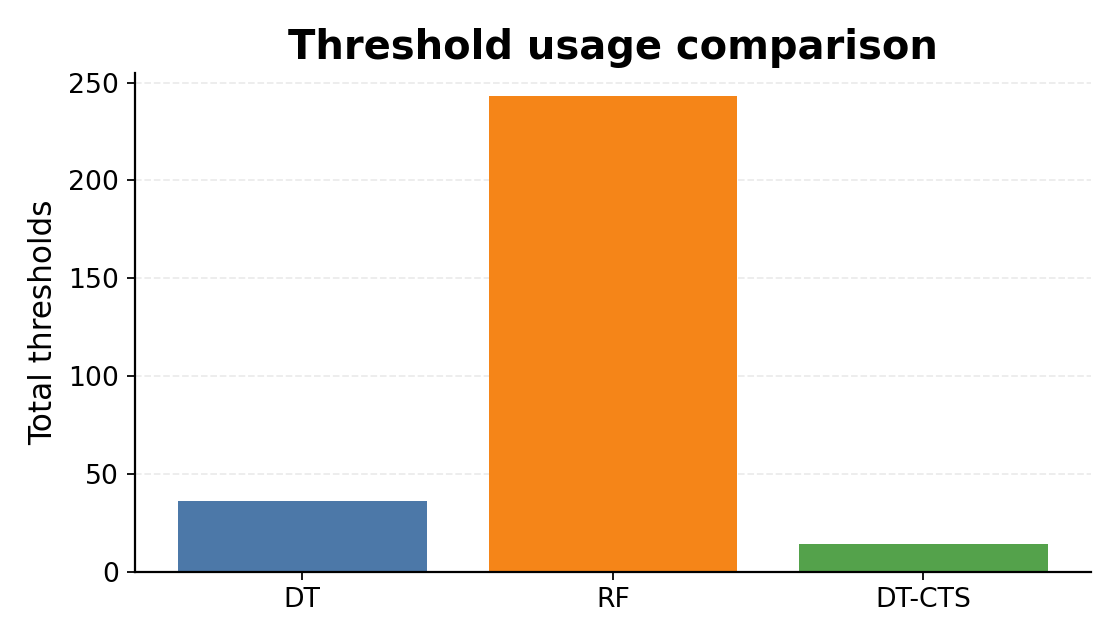
\includegraphics[width=\textwidth]{figures/threshold_usage.png}
    \caption{Threshold usage trong reproduction chính.}
    \label{fig:threshold-usage}
\end{subfigure}\hfill
\begin{subfigure}[t]{0.48\textwidth}
    \centering
    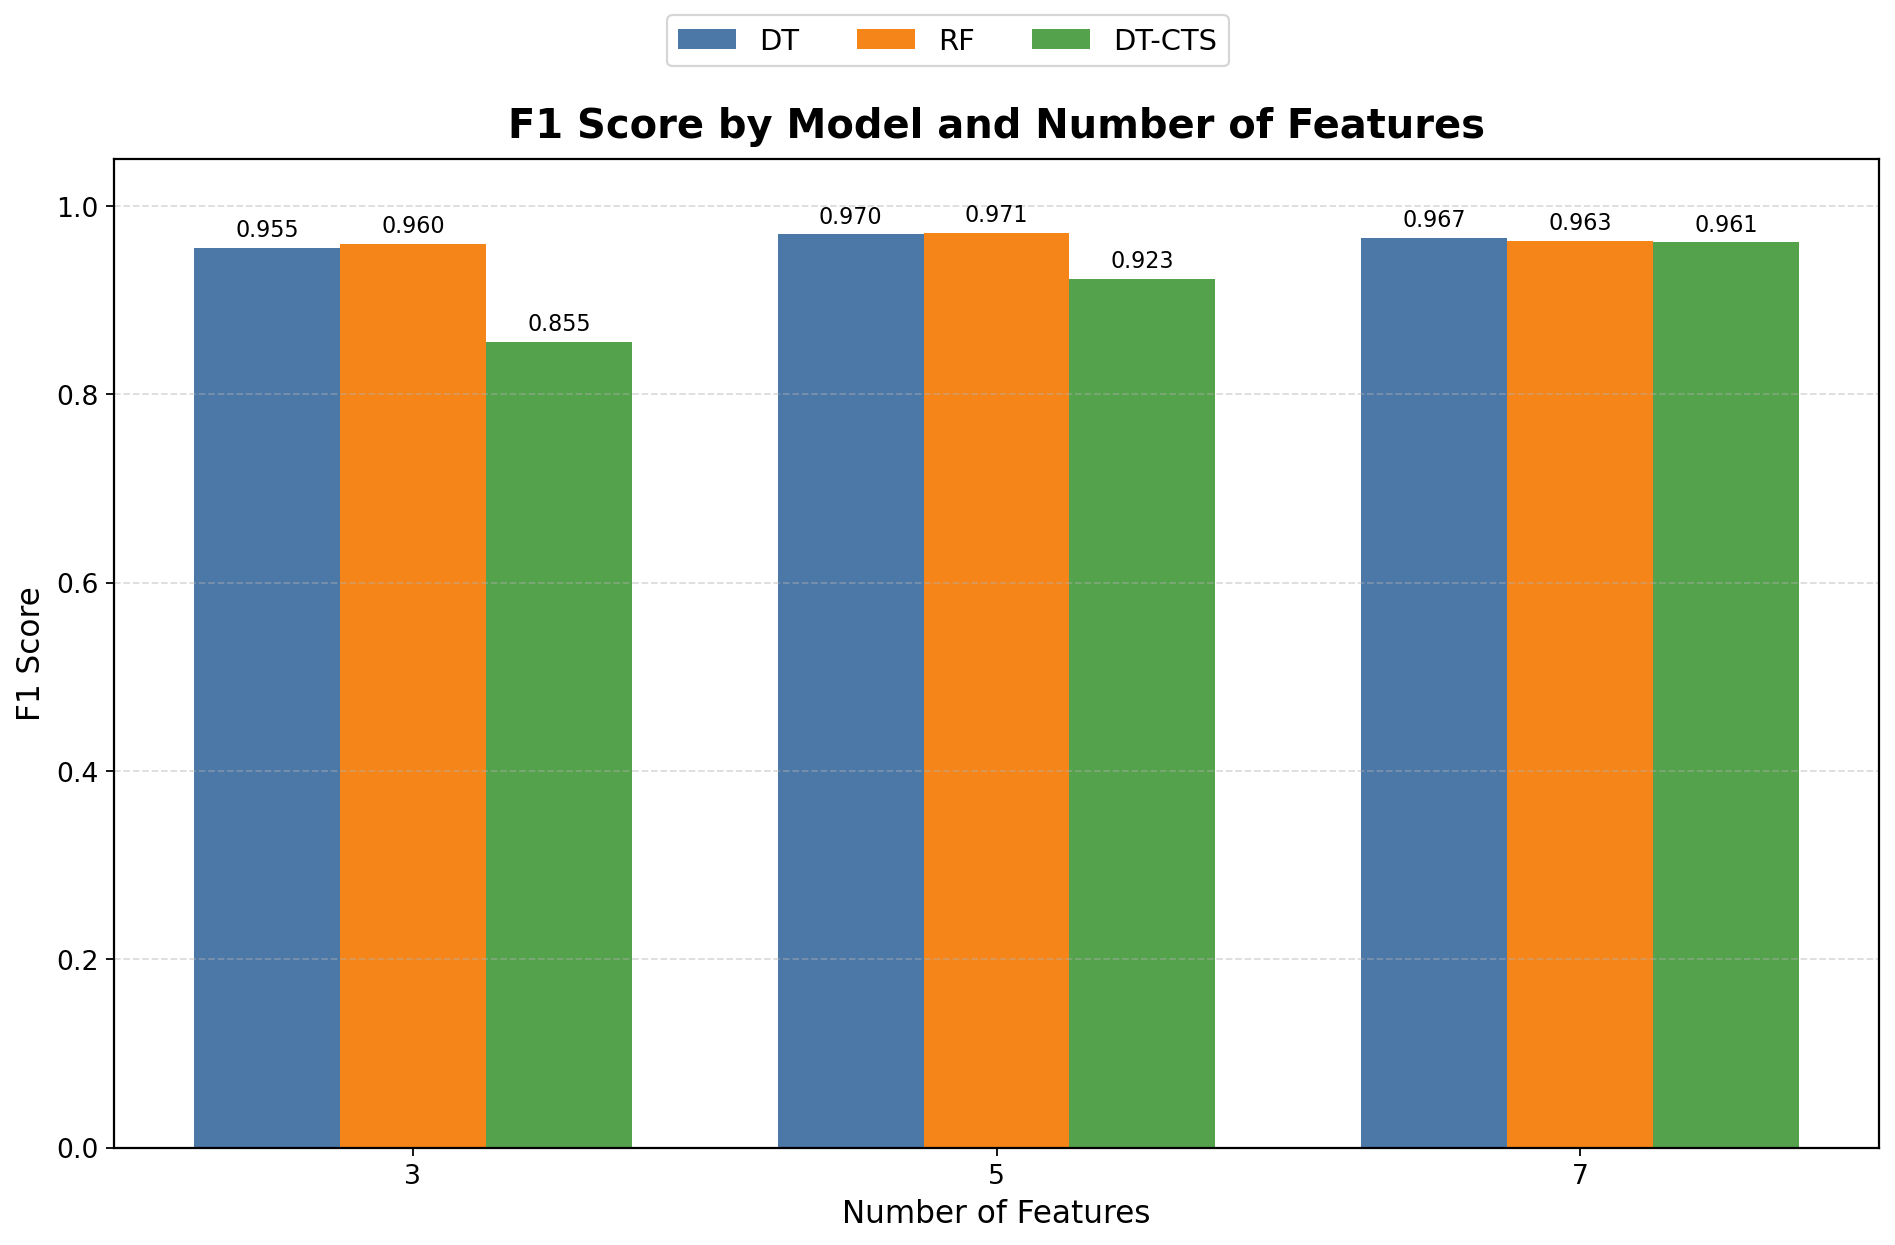
\includegraphics[width=\textwidth]{figures/benchmark_f1_scores.png}
    \caption{F1 trong benchmark paper-style với 3/5/7 feature.}
    \label{fig:benchmark-f1}
\end{subfigure}
\caption{So sánh trade-off giữa chất lượng và footprint. DT-CTS duy trì chất lượng đủ tốt trong khi giảm đáng kể số threshold.}
\label{fig:threshold-benchmark-pair}
\end{figure}

\subsection{Đánh giá cơ chế pushback mới}

\begin{table}
\caption{So sánh ba policy pushback trong thí nghiệm cải tiến.}
\label{tab:pushback-compare}
\centering
\begin{tabular}{lrrc}
\toprule
\textbf{Policy} & \textbf{Attack bytes} & \textbf{Benign bytes} & \textbf{False blocks} \\
\midrule
No pushback & 5{,}876{,}251 & 2{,}196{,}901{,}718 & 0 \\
Immediate pushback & 0 & 1{,}760{,}928{,}313 & 11 \\
Hierarchical pushback & 4{,}591 & 2{,}052{,}047{,}683 & 0 \\
\bottomrule
\end{tabular}
\end{table}

Trong phần giảm thiểu, project so sánh ba policy:
\begin{enumerate}
\item \texttt{no\_pushback}: không giảm thiểu upstream.
\item \texttt{immediate\_pushback}: block ngay sau một lần phát hiện malicious.
\item \texttt{hierarchical\_confidence\_pushback}: policy cải tiến của nhóm.
\end{enumerate}

Kết quả nổi bật như sau:
\begin{itemize}
\item \texttt{no\_pushback}: 5{,}876{,}251 attack bytes tới victim.
\item \texttt{immediate\_pushback}: attack bytes về 0 nhưng có 11 false block events.
\item \texttt{hierarchical\_confidence\_pushback}: chỉ còn 4{,}591 attack bytes tới victim và 0 false block events.
\end{itemize}

So với baseline không pushback, policy mới giảm khoảng 99.92\% attack bytes. Đồng thời, nó vẫn giữ được 2{,}052{,}047{,}683 benign bytes tới victim, cao hơn rõ rệt so với immediate pushback. Điều đó cho thấy phần cải tiến của project có giá trị thực tế: thay vì cố triệt tiêu attack bằng mọi giá, nó ưu tiên một điểm cân bằng tốt hơn giữa phòng thủ và tính sẵn sàng của traffic hợp lệ.

\begin{figure}
\centering
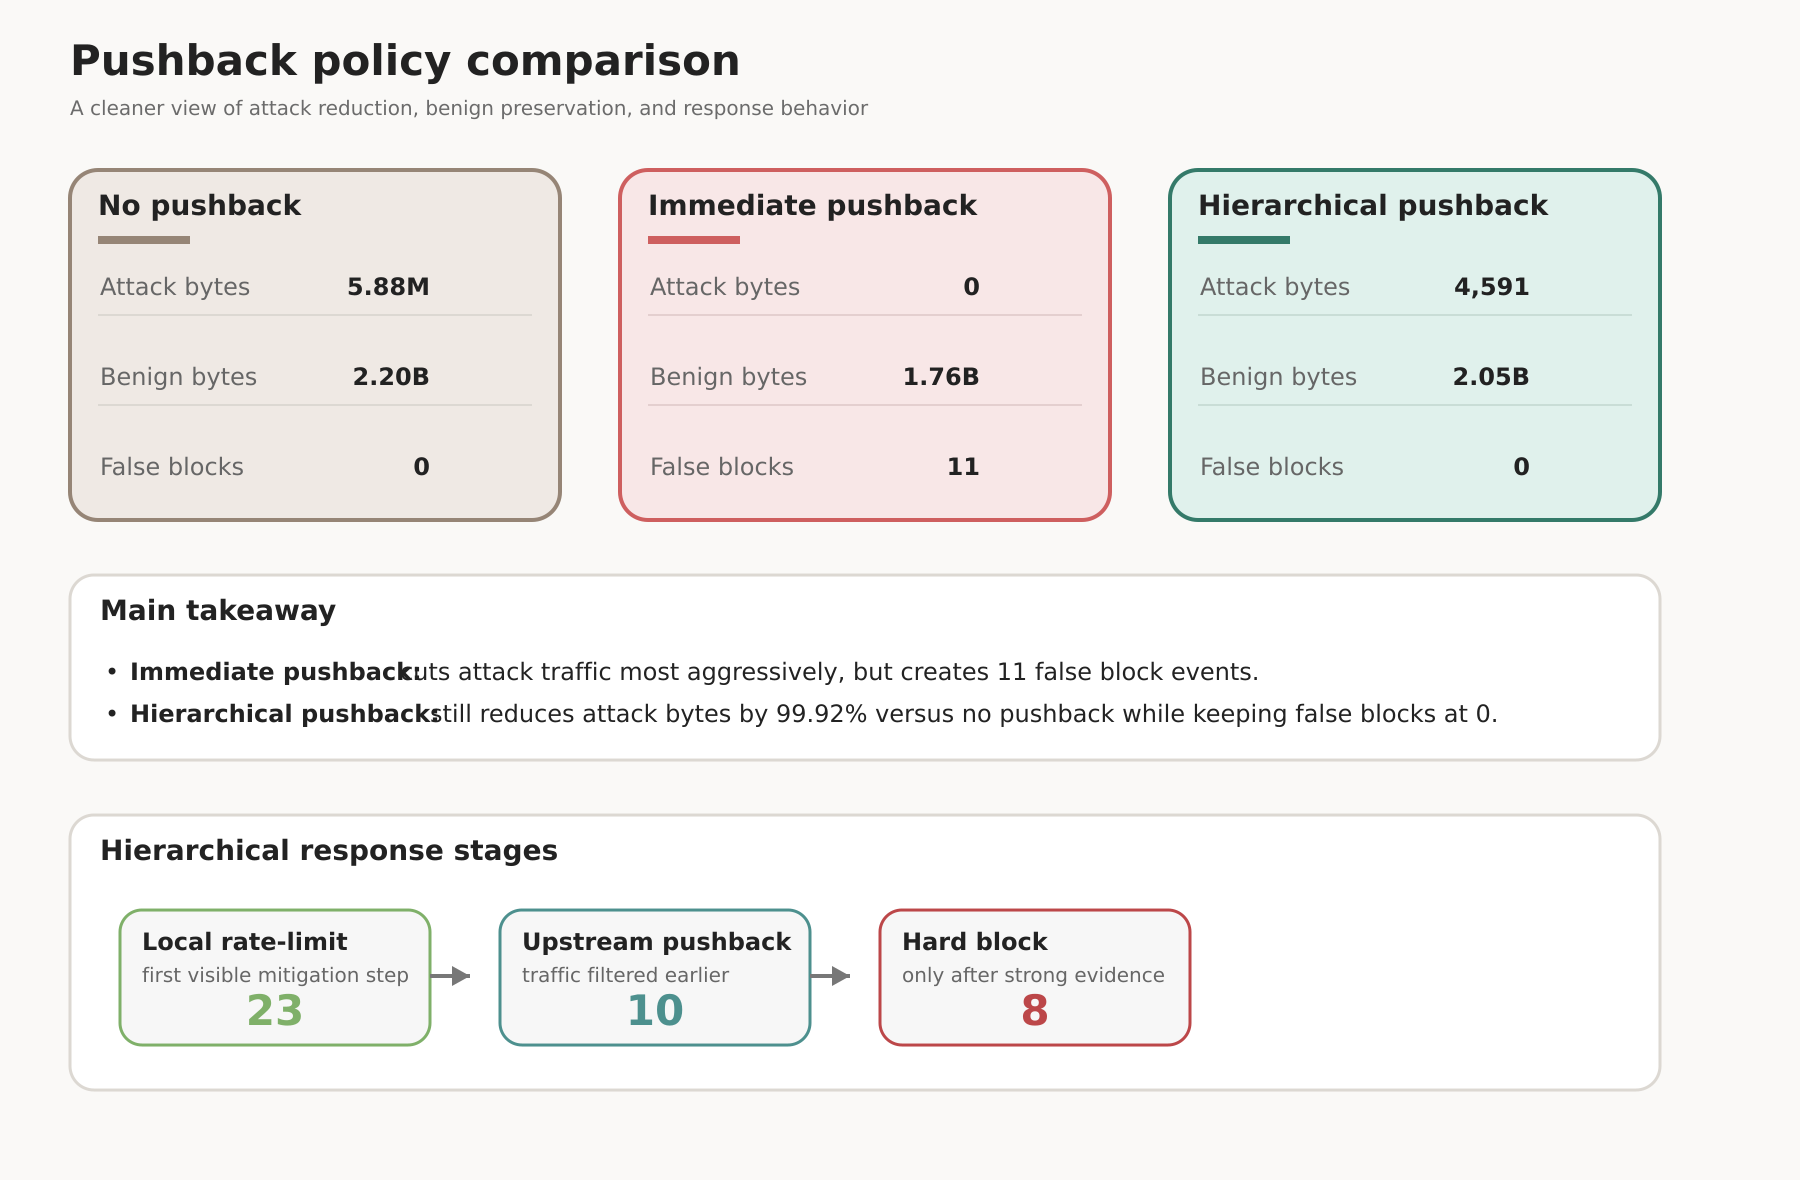
\includegraphics[width=0.95\textwidth]{figures/pushback_clean_summary.png}
\caption{Tóm tắt trực quan kết quả của ba policy pushback. Hình này chỉ giữ lại các thông tin quan trọng nhất: lượng attack traffic còn tới victim, lượng benign traffic được giữ lại, số lần false block và số lần leo thang ở policy cải tiến.}
\label{fig:pushback-clean-summary}
\end{figure}

\subsection{Phân tích hành vi leo thang}

Một điểm đáng chú ý là policy mới thực sự sử dụng các mức trung gian chứ không nhảy thẳng lên hard block. Trong lần chạy hiện tại, hệ thống ghi nhận 23 local rate-limit events, 10 upstream pushback events và 8 hard block events. Điều này cho thấy suspicion score thực sự đóng vai trò như một bộ nhớ trạng thái, giúp hệ thống đánh giá lại source qua nhiều window thay vì ra quyết định chỉ từ một dự đoán duy nhất.

\subsection{Thảo luận}

Từ các kết quả trên có thể rút ra ba nhận xét. Thứ nhất, DT-CTS là lựa chọn hợp lý khi mục tiêu bao gồm cả triển khai data plane chứ không chỉ dừng ở classification quality. Thứ hai, immediate pushback rất mạnh trong việc triệt tiêu attack nhưng lại quá nhạy với false positive. Thứ ba, hierarchical confidence-aware pushback giải quyết bài toán ở cấp hệ thống tốt hơn vì nó cho phép phản ứng theo mức, gần với cách một hệ thống thực tế nên vận hành.

Tất nhiên, báo cáo vẫn còn một số giới hạn. Các kết quả pushback hiện mới được đo trong mô phỏng flow-level, chưa phải trên mạng thật hoặc ASIC thật. Ngoài ra, threshold count cũng chỉ là chỉ báo gián tiếp cho footprint phần cứng. Dù vậy, các kết quả hiện tại vẫn đủ để cho thấy hướng cải tiến của nhóm là hợp lý và có ý nghĩa hơn một thay đổi nhỏ ở ngưỡng block.

\section{Kết luận}

Nghiên cứu đã tái hiện rút gọn các ý chính của SISTAR trong một workflow phần mềm có thể chạy lại, bao gồm phát hiện DDoS bằng mô hình cây quyết định nhẹ, so sánh số threshold như một chỉ báo cho khả năng triển khai và mô phỏng cơ chế pushback để đánh giá tác động tới victim. Kết quả cho thấy DT-CTS là mô hình phù hợp với mục tiêu nghiên cứu vì vẫn duy trì được chất lượng cạnh tranh trong khi giảm mạnh độ phức tạp so với cây quyết định thông thường.

Đóng góp quan trọng hơn nằm ở phần cải tiến hệ thống: hierarchical confidence-aware pushback. Cơ chế này thay thế cách block ngay bằng một quá trình tích lũy bằng chứng từ edge detector, core detector và tín hiệu spike, sau đó mới leo thang phản ứng qua bốn mức. Nhờ đó, hệ thống vẫn làm giảm gần như toàn bộ attack traffic tới victim nhưng tránh được false block trong mô phỏng hiện tại.

Trong tương lai, một hướng mở rộng hợp lý là chuyển từ mô phỏng flow-level sang đánh giá thực hơn trên BMv2 hoặc môi trường P4 có thể đo trực tiếp chi phí bảng match, register và độ trễ xử lý. Bên cạnh đó, policy mới cũng có thể được tinh chỉnh thêm bằng các chiến lược học ngưỡng động theo tải mạng hoặc theo từng nhóm nguồn lưu lượng.



\begin{credits}
\subsubsection{Source code/Dataset} Source code and experiment outputs are taken from the accompanying project repository. The main dataset view used in this study is the paper-compatible BENIGN vs Wednesday DoS subset derived from CICIDS2017.
\end{credits}
\FloatBarrier
\clearpage
%
% ---- Bibliography ----
%
% BibTeX users should specify bibliography style 'splncs04'.
% References will then be sorted and formatted in the correct style.
%
\bibliographystyle{splncs04}
\bibliography{references}
\end{document}
